\section{Regression Function Estimation}
\subsection{Introduction: average effect of $X$ on $Y$}
The model for a nonparametric model is $$Y=f(X)+\varepsilon$$, where
$\E\bra{\varepsilon|X}=0$ and $\E\bra{\abs{\varepsilon}}<\infty$. The goal is
to estimate $f$. We say it has a random design if $X$ is random, and a fixed
design if $X$ is fixed. We will focus on the random design case. \\First, we
define the average effect of $X$ on $Y$ as $\E\bra{f\pa{X}}$ if the expectation
is defined. \\If $f_{y\mid x}$, the conditional density of $Y$ given $X$
exists, it is given by $f_{Y\mid X}\pa{y\mid x} = \frac{f\pa{x,y}}{f_X\pa{x}}$
if $f_X\pa{x}>0$. Also the conditional expectation function $\E\bra{Y|X=x}$ is
given by $$\E\bra{Y|X=x}= \int y f_{Y\mid X}\pa{y\mid x}dy = \frac{\int y
        f\pa{x,y}dy}{f_X(x)}=\frac{\int y f\pa{x,y}dy}{\int f\pa{x,y}dy}.$$ A\ natural
idea would be to use $$ \hat{f}_X(x) = \frac{1}{nh^2}\sum_{i=1}^n
    K\pa{\frac{X_i-x}{h}}K\pa{\frac{Y_i-y}{h}},$$ where $K$ is a kernel.

As an exercise, we can check that $$\int y \hat{f}_{Y,X}\pa{y,x}dy =
    \frac{1}{nh}\sum_{i=1}^n K\pa{\frac{X_i-x}{h}}Y_i$$ and $$\int
    \hat{f}_{Y,X}\pa{y,x}dy = \frac{1}{nh}\sum_{i=1}^n K\pa{\frac{X_i-x}{h}}.$$
\subsection{Nadaraya-Watson estimator}
This leads to the following estimator called \textbf{Nadaraya-Watson estimator}
$$\hat{f}_X(x) = \frac{\sum_{i=1}^n K\pa{\frac{X_i-x}{h}}Y_i}{\sum_{i=1}^n
        K\pa{\frac{X_i-x}{h}}}.$$ In practice, dealing with the denominator can be
tricky. We propose two ideas to deal with this issue.
\begin{enumerate}
    \item We can work with \textbf{nonnegative} kernels because \begin{equation*}
              \sum Y_i \underbrace{\frac{K\pa{\frac{X_i-x}{h}}}{\sum_{i=1}^n K\pa{\frac{X_i-x}{h}}}}_{\in \bra{0,1}}.
          \end{equation*}
    \item We can use a trimming factor $\rho$ and write $$\hat{f}_X(x) =
              \frac{\sum_{i=1}^n K\pa{\frac{X_i-x}{h}}Y_i}{\max\pa{\sum_{i=1}^n
                      K\pa{\frac{X_i-x}{h}},\rho}}.$$
\end{enumerate}
Suppose now $\text{supp}\pa{X}=[a,b]$ and $\exists\ m>0\ \text{s.t.}\ f_X(x)\ge m$. Suppose I am interested in $f\pa{b}$ and I use the rectangular kernel \ref{ker:rect}.
\begin{figure*}[!h]
    \centering
    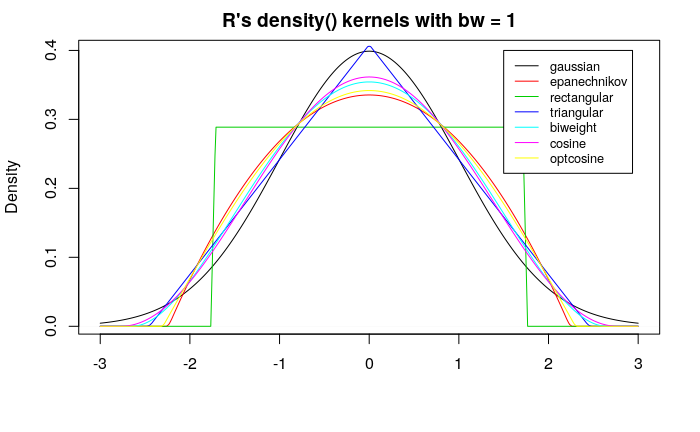
\includegraphics[width=0.8\textwidth]{figures/kernels.png}
    \caption{Kernels}
\end{figure*}
Then $\hat{f}\pa{b}$ where $\hat{f}$ is the N.W. estimator is biased. But a local polynomial estimator of order $\ge 1$ is consistent and unbiased.
\begin{remark}
    In TD, we will see that we can get a fast rate of convergence with nonnegative kernels (unlike in density estimation).
\end{remark}
\subsection{Local Polynomial Estimation}
\textit{tutorial 3}